% Provenance (never printed): see sources/outline_sources.md (Year 3: gravitational
% potential, spherical harmonics, J2, reference ellipsoid, geoid, satellite gravimetry,
% flexure of the lithosphere). Brief: sources/book5/BRIEFS.md, ch. 3. Curves from
% figdata/bachelor-3/hydrostatic_figure.py, ice_mass.py (IMBIE 2021), flexure.py.
% Exercise and problem values in the Book 5 scratch calculator calc/ch03.py.
\chapter{Zwaartekracht en de vorm van de Aarde}\label{ch:b3:gravity-geodesy}

Twee satellieten vliegen achter elkaar om de Aarde, op een hoogte van meer
dan \qty{500}{km} en ongeveer \qty{220}{km} van elkaar, en meten de afstand
onderling voortdurend, tot op een micrometer nauwkeurig.
% ledger: geod5:grace, geod5:grace-ranging
Wanneer ze boven een plek vliegen waar massa is geconcentreerd, wordt eerst de voorste satelliet
naar voren getrokken en de tussenruimte gaat open; daarna wordt de achterste op zijn beurt
aangetrokken en de tussenruimte sluit zich. Uit die minieme veranderingen, maand na maand sinds 2002,
is het zwaartekrachtsveld van de Aarde in kaart gebracht zoals het verandert: het water dat
in stroomgebieden is opgeslagen, stijgt en daalt met de seizoenen, en de grote ijskappen van
Groenland en Antarctica verliezen jaar na jaar massa. Zwaartekracht weegt wat het oog
niet kan zien. Dit hoofdstuk bouwt het zwaartekrachtsveld van een roterende planeet op uit
zijn potentiaal, vindt daarin de afplatting en het traagheidsmoment, volgt zijn
anomalieën tot in de baan, en wendt zich dan tot een van de dingen die zwaartekracht
aan het oppervlak onthult: de buiging van de lithosfeer onder het gewicht van een vulkaan.

\begin{recall}
De gravitatiewet van Newton, de gravitatiepotentiële energie en de
centrifugaalkracht in een roterend assenstelsel komen uit de natuurkundeboeken; de traagheidsmomenten van
een vast lichaam en de Legendre-polynomen $P_2(x) = (3x^2 - 1)/2$ staan in
de universitaire delen van de natuurkunde- en wiskundeboeken, de elasticiteitsmodulus van Young $E$ en
de dwarscontractiecoëfficiënt van Poisson $\nu$ in het derde-jaarsdeel van de natuurkundeboeken. Geodesie en de
afplatting $f = (a - b)/a$ van een ellipsoïde met halve assen $a > b$ kwamen aan de orde in
leerjaar~10. Isostasie, Airy-compensatie, normale zwaartekracht, de geoïde, de geoïdehoogte
en de zwaartekrachtsanomalieën werden gedefinieerd in Boek~3, in het hoofdstuk
over isostasie en zwaartekrachtsanomalieën.
\end{recall}

\section{De geopotentiaal}

Op een roterende planeet voelt een lichaam in rust de aantrekking van de massa van de planeet
en, in het assenstelsel dat met de planeet meedraait, de centrifugaalkracht. Beide zijn afgeleid
van een potentiaal.

\begin{definition}[Geopotentiaal]\label{def:b3:gravity-geodesy:geopotential}
De \emph{geopotentiaal}\index{geopotentiaal} is de potentiële energie per eenheid van
massa, in het assenstelsel dat met de Aarde meedraait met de hoeksnelheid $\omega$, van
de gravitatie en de centrifugaalkracht samen:
\[
  W(\mathbf r) = V(\mathbf r) + \Phi(\mathbf r),\qquad
  V(\mathbf r) = -G\int_{\text{Aarde}}\frac{\mathrm dm'}{|\mathbf r - \mathbf r'|},\qquad
  \Phi(\mathbf r) = -\tfrac12\omega^2 s^2,
\]
waarin $s$ de afstand tot de rotatieas is. De zwaartekracht is
$\mathbf g = -\nabla W$, en de oppervlakken $W = \text{constant}$ zijn haar
niveauoppervlakken: overal staat de zwaartekracht loodrecht op ze.
\end{definition}

Een schietlood hangt langs $-\nabla W$, en stilstaand water komt tot rust op een
niveauoppervlak. Een roterende vloeibare planeet neemt daarom de vorm aan van een van zijn eigen
niveauoppervlakken: de centrifugaalpotentiaal, die aan de evenaar het diepst is, zwelt de
evenaar op en vlakt de polen af.

\begin{omfigure}
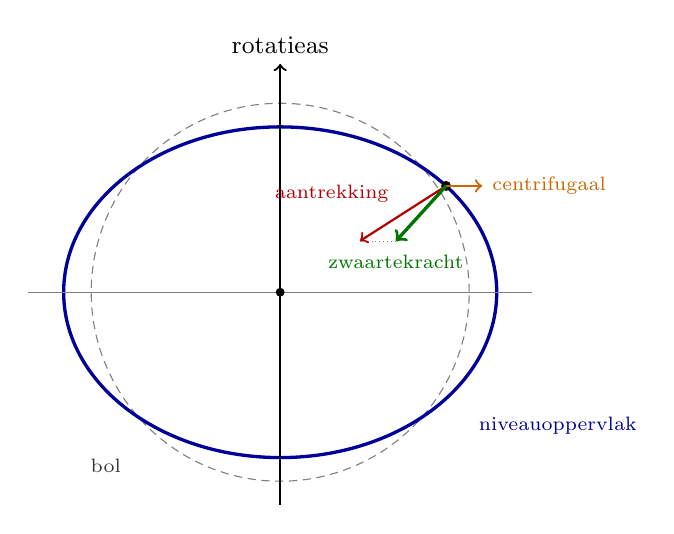
\begin{tikzpicture}[font=\small, x=1cm, y=1cm]
\draw[gray, densely dashed] (0,0) circle (2.4);
\draw[very thick, blue!60!black] (0,0) ellipse (2.75 and 2.1);
\draw[->, thick] (0,-2.7) -- (0,2.9) node[above] {rotatieas};
\draw[gray] (-3.2,0) -- (3.2,0);
\fill (0,0) circle (1.6pt);
% a point at latitude 40 deg (parameter) on the ellipse; the attraction points at
% the centre, the centrifugal force is horizontal, and their sum is drawn along the
% inward normal of the ellipse: lengths solved so that the sum is normal (calc/ch03_fig.py)
\coordinate (P) at (2.107,1.350);
\fill (P) circle (1.8pt);
\draw[->, thick, red!70!black] (P) -- (1.012,0.650);
\node[font=\scriptsize, red!70!black, anchor=south east] at (1.50,1.02) {aantrekking};
\draw[->, thick, orange!80!black] (P) -- (2.565,1.350) node[right, font=\scriptsize] {centrifugaal};
\draw[gray, densely dotted] (1.012,0.650) -- (1.470,0.650);
\draw[->, very thick, green!45!black] (P) -- (1.470,0.650);
\node[font=\scriptsize, green!45!black, anchor=north] at (1.470,0.600) {zwaartekracht};
\node[blue!60!black, anchor=west, font=\scriptsize] at (2.4,-1.7) {niveauoppervlak};
\node[gray!40!black, anchor=east, font=\scriptsize] at (-1.9,-2.2) {bol};
\end{tikzpicture}

\par\smallskip{\small Een niveauoppervlak van een roterende planeet (schematisch, de
afplatting sterk overdreven). Op elk punt staat de zwaartekracht, de som van de
aantrekking en de centrifugaalkracht, loodrecht op het niveauoppervlak; zij wijst
niet naar het middelpunt, behalve aan de polen en op de evenaar.}
\label{fig:b3:gravity-geodesy:equipotential}
\end{omfigure}

Buiten de planeet voldoet het gravitatiepotentiaal aan de vergelijking van Laplace, en
de oplossingen die regulier zijn in oneindig, zijn de solide sferische harmonischen.

\begin{proposition}[Ontwikkeling van de geopotentiaal in sferische harmonischen]\label{prop:b3:gravity-geodesy:harmonics}
Buiten een lichaam met massa $M$ en equatoriale straal $a$, met de oorsprong in zijn
massamiddelpunt en de $z$-as langs zijn rotatieas, is de gravitatiepotentiaal
op afstand $r$, colatitude $\theta$ en lengtegraad $\lambda$ gegeven door
\begin{multline*}
  V = -\frac{GM}{r}\Biggl[1 - \sum_{n=2}^{\infty}\left(\frac ar\right)^nJ_nP_n(\cos\theta)\\
  + \sum_{n=2}^{\infty}\sum_{m=1}^{n}\left(\frac ar\right)^nP_{nm}(\cos\theta)
  (C_{nm}\cos m\lambda + S_{nm}\sin m\lambda)\Biggr],
\end{multline*}
met de Legendre-polynomen $P_n$ en de geassocieerde functies $P_{nm}$; de
coëfficiënten $J_n$, $C_{nm}$, $S_{nm}$ zijn getallen die aan waarnemingen zijn aangepast. Voor
een lichaam dat symmetrisch is om zijn as, blijven alleen de zonale termen $J_n$ over. Geen term van
graad 1 komt voor.
\end{proposition}

\begin{proof}
De scheiding van variabelen in de vergelijking van Laplace in bolcoördinaten
levert de in oneindig reguliere oplossingen $r^{-(n+1)}P_{nm}(\cos\theta)e^{\pm
im\lambda}$ (de universitaire delen van de wiskundeboeken); elke potentiaal buiten
de massa's is een som ervan. De term van graad 0 is $-GM/r$, de potentiaal van
de gehele massa. De termen van graad 1 zijn evenredig met de eerste momenten
$\int\mathbf r'\,\mathrm dm'$, die verdwijnen als de oorsprong in het
massamiddelpunt ligt. Axiale symmetrie schrapt elke term die van $\lambda$ afhangt.
\end{proof}

\begin{definition}[Dynamische vormfactor]\label{def:b3:gravity-geodesy:j2}
De \emph{dynamische vormfactor}\index{dynamische vormfactor} $J_2$ van een planeet
is de coëfficiënt van zijn zonale harmonische van graad 2: de grootste afwijking van
zijn externe potentiaal ten opzichte van die van een bol, veroorzaakt door zijn afplatting. Voor de
Aarde geldt $J_2 = \num{1.08263e-3}$.
% ledger: geod5:grs80-defining
\end{definition}

\begin{theorem}[Formule van MacCullagh]\label{thm:b3:gravity-geodesy:maccullagh}
Laat $A$, $B$, $C$ de hoofdtraagheidsmomenten zijn van een lichaam met massa $M$
om assen door zijn massamiddelpunt, en $I$ zijn traagheidsmoment om de
lijn van het massamiddelpunt naar een extern punt op afstand $r$. Tot en met
orde $r^{-3}$ wordt de gravitatiepotentiaal in dat punt gegeven door de
\emph{formule van MacCullagh}\index{formule van MacCullagh}
\[
  V = -\frac{GM}{r} - \frac{G(A + B + C - 3I)}{2r^3} .
\]
Voor een lichaam dat symmetrisch is om de $z$-as ($A = B$),
$V = -\dfrac{GM}{r} + \dfrac{G(C - A)}{r^3}P_2(\cos\theta)$, zodat
\[
  J_2 = \frac{C - A}{Ma^2} .
\]
\end{theorem}

\begin{proof}
Met $\hat{\mathbf r}$ de eenheidsvector naar het punt en $r' \ll r$,
\[
  \frac{1}{|\mathbf r - \mathbf r'|} = \frac1r + \frac{\hat{\mathbf r}\cdot\mathbf r'}{r^2}
  + \frac{3(\hat{\mathbf r}\cdot\mathbf r')^2 - r'^2}{2r^3} + O(r^{-4}).
\]
Geïntegreerd over de massa geeft de eerste term $M/r$, en de tweede verdwijnt
(massamiddelpunt). Voor de derde geldt $\int r'^2\,\mathrm dm' = (A + B + C)/2$, omdat
$A + B + C = \int 2r'^2\,\mathrm dm'$, en $\int(\hat{\mathbf r}\cdot\mathbf
r')^2\,\mathrm dm' = \int r'^2\,\mathrm dm' - I$, want het kwadraat van de afstand tot
de lijn is $r'^2 - (\hat{\mathbf r}\cdot\mathbf r')^2$. De haakjesterm integreert
tot $3(A + B + C)/2 - 3I - (A + B + C)/2 = A + B + C - 3I$. Voor $A = B$ is het
traagheidsmoment om een lijn op co-breedte $\theta$ gelijk aan $I = A\sin^2\theta + C\cos^2\theta$,
en $2A + C - 3I = (C - A)(1 - 3\cos^2\theta) = -2(C - A)P_2(\cos\theta)$.
Vergelijken met \cref{prop:b3:gravity-geodesy:harmonics} geeft
$J_2Ma^2 = C - A$.
\end{proof}

De term van graad 2 van de potentiaal meet dus het verschil van de
traagheidsmomenten, niet de momenten zelf. De precessie van de aardas, aangedreven door de
koppels van de Zon en de Maan op de equatoriale uitstulping,
meet de dynamische elliptiteit $H = (C - A)/C$; samen geven $J_2$ en $H$ de
$C/(Ma^2)$, de traagheidsmomentfactor, \num{0.3308} voor de Aarde,
% ledger: earth:MoI
duidelijk lager dan de \num{0.4} van een homogene bol: de massa is naar het
middelpunt geconcentreerd.

\section{De roterende ellipsoïde}

\begin{definition}[Referentie-ellipsoïde]\label{def:b3:gravity-geodesy:ellipsoid}
Een \emph{referentie-ellipsoïde}\index{referentie-ellipsoïde} is een ellipsoïde van
omwenteling, met equatoriale halve as $a$ en afplatting $f$, zo gekozen dat het
zelf een niveauoppervlak is van een modelpotentiaal: de potentiaal van een roterend
lichaam met massa $M$, hoeksnelheid $\omega$ en de \omterm{def:b3:gravity-geodesy:j2}{dynamische vormfactor}
$J_2$ van de Aarde. Vier constanten bepalen haar; het Geodetic Reference
System 1980 neemt
\begin{gather*}
  a = \qty{6378137}{m},\qquad GM = \qty{3.986005e14}{m^3.s^{-2}},\\
  J_2 = \num{1.08263e-3},\qquad \omega = \qty{7.292115e-5}{rad.s^{-1}},
\end{gather*}
en leidt daaruit de afplatting $f = \num{0.00335281068}$
($1/f = \num{298.257222}$) en de kleine halve as
$b = \qty{6356752.3141}{m}$ af.
% ledger: geod5:grs80-defining, geod5:grs80-derived
\end{definition}

De potentiaal van het model, de normale potentiaal, is in gesloten vorm bekend, en
evenzo de zwaartekracht ervan op de ellipsoïde, de normale zwaartekracht uit Boek~3.

\begin{proposition}[Formule van Somigliana]\label{prop:b3:gravity-geodesy:somigliana}
Op een \omterm{def:b3:gravity-geodesy:ellipsoid}{referentie-ellipsoïde} met halve assen $a$, $b$ en normale zwaartekracht
$\gamma_e$ aan de evenaar en $\gamma_p$ aan de polen, wordt de normale zwaartekracht op de
geodetische breedte $\varphi$ gegeven door de \emph{formule
van Somigliana}\index{formule van Somigliana}
\[
  \gamma(\varphi) = \frac{a\gamma_e\cos^2\varphi + b\gamma_p\sin^2\varphi}
  {\sqrt{a^2\cos^2\varphi + b^2\sin^2\varphi}} .
\]
Voor het Geodetic Reference System 1980 geldt $\gamma_e = \qty{9.7803267715}{m.s^{-2}}$
en $\gamma_p = \qty{9.8321863685}{m.s^{-2}}$, en de reeks
$\gamma = 9.780327(1 + 0.0053024\sin^2\varphi - 0.0000058\sin^22\varphi)$
\unit{m.s^{-2}} reproduceert de formule tot op \qty{0.1}{\milli\gal}.
% ledger: geod5:grs80-derived, moritz:grs80 (Book 3, read-only)
\end{proposition}
\admitted

Hoe plat moet een roterende planeet zijn? Als het een vloeistof in hydrostatisch
evenwicht is, wordt de afplatting vastgelegd door zijn rotatie en door hoe zijn massa
over de diepte is verdeeld.

\begin{proposition}[Relaties van Clairaut en Darwin--Radau]\label{prop:b3:gravity-geodesy:clairaut}
Voor een planeet in hydrostatisch evenwicht, met $m = \omega^2a^2b/(GM)$ de verhouding
van de centrifugale tot de gravitatieversnelling aan de evenaar, tot in de eerste
orde in $f$ en $m$:
\[
  J_2 = \frac{2f - m}{3}\qquad\text{(Clairaut)},\qquad
  \frac{C}{Ma^2} = \frac23\left[1 - \frac25\sqrt{\frac52\frac mf - 1}\right]
  \qquad\text{(Darwin--Radau)} .
\]
Een homogene planeet ($C/Ma^2 = 0.4$) heeft $f = 5m/4$; een planeet waarvan de massa
naar het middelpunt geconcentreerd is, is minder afgeplat.
\end{proposition}
\admitted

Met de relatie van Clairaut en de $m = \num{0.00344979}$ van de Aarde wordt de gemeten
$J_2$ omgezet in $f = \num{0.0033488}$, of $1/298.6$: binnen
\qty{0.12}{\percent} van de afplatting van de ellipsoïde. De relatie van Darwin--Radau
geeft, met de traagheidsmomentfactor, de afplatting die de Aarde zou hebben als zij
een vloeistof in evenwicht was: $1/299.9$, tegenover de gemeten
$1/298.26$. De Aarde is iets platter dan een vloeistofplaneet met haar rotatie
en haar massaverdeling zou hebben: haar equatoriale uitstulping ligt ongeveer
\qty{116}{m} hoger dan het hydrostatisch evenwicht voorspelt. De Aarde is niet
exact een vloeistof in evenwicht, en het kleine verschil is zelf een
meting van de spanningen die haar inwendige draagt.

\begin{omfigure}
\begin{tikzpicture}
\begin{axis}[omrecord, width=0.74\linewidth, height=0.44\linewidth,
  xmin=0.3, xmax=0.4, ymin=225, ymax=340,
  xlabel={traagheidsmomentfactor $C/(Ma^2)$}, ylabel={hydrostatisch $1/f$},
  xtick={0.30,0.32,0.34,0.36,0.38,0.40},
  xticklabel style={/pgf/number format/fixed, /pgf/number format/precision=2}]
\addplot[blue!70!black, thick] table[x=moi, y=f_inv] {figdata/out/bachelor-3-hydrostatic_figure-curve.dat};
\draw[gray, densely dashed] (axis cs:0.3308,225) -- (axis cs:0.3308,299.88);
\draw[gray, densely dashed] (axis cs:0.3,299.88) -- (axis cs:0.3308,299.88);
\fill[blue!70!black] (axis cs:0.3308,299.88) circle (2pt);
\node[font=\scriptsize, anchor=south west] at (axis cs:0.3315,301) {hydrostatische Aarde, $1/f = 299.9$};
\draw[red!70!black, thick] (axis cs:0.3,298.26) -- (axis cs:0.4,298.26);
\node[font=\scriptsize, anchor=north east, red!70!black] at (axis cs:0.399,296.5) {waargenomen, $1/f = 298.26$};
\fill (axis cs:0.4,231.9) circle (2pt);
\node[font=\scriptsize, anchor=east] at (axis cs:0.397,233) {uniforme planeet};
\end{axis}
\end{tikzpicture}

\par\smallskip{\small De afplatting van een vloeistofplaneet met de rotatie van de Aarde,
uitgezet tegen haar traagheidsmomentfactor, volgens de relatie van Darwin--Radau
(berekend met het Geodetic Reference System 1980). Hoe meer de massa
naar het centrum is geconcentreerd, hoe ronder de planeet. Voor de Aarde
met \num{0.3308} bedraagt de hydrostatische afplatting $1/299.9$, iets minder dan de
waargenomen $1/298.26$.}
\label{fig:b3:gravity-geodesy:hydrostatic}
\end{omfigure}

\section{De geoïde en de storingspotentiaal}

De geoïde is het niveauoppervlak van de werkelijke \omterm{def:b3:gravity-geodesy:geopotential}{geopotentiaal} dat samenvalt met
het gemiddelde zeeniveau; het \omterm{def:b3:gravity-geodesy:ellipsoid}{referentie-ellipsoïde} is een niveauoppervlak van de normale
potentiaal $U$ met dezelfde waarde, $U_0 = W_0$. Hun scheiding, de geoïdehoogte $N$,
wordt bepaald door het verschil van de twee potentialen.

\begin{proposition}[Formule van Bruns]\label{prop:b3:gravity-geodesy:bruns}
Laat $T = W - U$ de storingspotentiaal zijn. De geoïdehoogte op een punt wordt
gegeven door de \emph{formule van Bruns}\index{formule van Bruns}
\[
  N = -\frac{T}{\gamma},
\]
waarbij $T$ op de geoïde wordt geëvalueerd en $\gamma$ de normale zwaartekracht daar is. Een
massaoverschot, dat de potentiaal verdiept ($T < 0$), tilt de geoïde op.
\end{proposition}

\begin{proof}
Laat P op de geoïde liggen en Q het punt van het ellipsoïde eronder, op de afstand
$N$. Omdat $U$ naar buiten toe toeneemt met de snelheid $\gamma$,
$U(\mathrm P) = U(\mathrm Q) + \gamma N = U_0 + \gamma N$. Dan
$W_0 = W(\mathrm P) = U(\mathrm P) + T(\mathrm P) = U_0 + \gamma N + T$, en
$W_0 = U_0$ geeft $N = -T/\gamma$.
\end{proof}

Een geoïdehoogte van \qty{50}{m} komt overeen met een potentiaalverschil van slechts
\qty{490}{J.kg^{-1}}, één deel op \num{e5} van de \omterm{def:b3:gravity-geodesy:geopotential}{geopotentiaal}. De
geoïdehoogten van de Aarde lopen van ongeveer $+\qty{85}{m}$ bij IJsland tot
$-\qty{106}{m}$ in Zuid-India,
% ledger: nasa:geoid-range (Book 3, read-only)
een spreiding van minder dan \qty{200}{m} op een planeet waarvan de equatoriale en poolstralen
\qty{21}{km} verschillen.

\section{Satellietgravimetrie}

\begin{definition}[Satellietgravimetrie]\label{def:b3:gravity-geodesy:satgrav}
\emph{Satellietgravimetrie}\index{satellietgravimetrie} bepaalt het zwaartekrachtveld van de Aarde
uit de beweging van satellieten: uit de langdurige storingen
van hun banen, uit de veranderende afstand tussen twee satellieten in dezelfde
baan, of met gradiometers die de verschillen in zwaartekracht over het
ruimtevaartuig meten.
\end{definition}

De grootste storing van een baan dicht bij de Aarde komt van $J_2$. De
equatoriale uitstulping oefent een koppel uit op de schuine baan, die langzaam
rond de aardas draait.

\begin{proposition}[Precessie van de knooplijn]\label{prop:b3:gravity-geodesy:nodal}
In eerste orde in $J_2$ draait de knooplijn van een cirkelbaan met straal $r$ en
inclinatie $i$ met de snelheid
\[
  \dot\Omega = -\frac32\,nJ_2\left(\frac ar\right)^2\cos i,\qquad n = \sqrt{GM/r^3} ,
\]
westwaarts voor een prograde baan ($i < \ang{90}$), oostwaarts voor een retrograde baan.
\end{proposition}

\begin{proof}
Over vele omwentelingen gedraagt de satelliet zich als een ring met massa $m_s$ die
over haar baan is uitgesmeerd. Het graad-2-deel van de potentiaal,
$(GMJ_2a^2/r^3)P_2(\cos\theta)$ per eenheid van massa, gemiddeld over een cirkel die
onder $i$ is geneigd, bevat $\langle\cos^2\theta\rangle = \tfrac12\sin^2i$, dus
$\langle P_2\rangle = \tfrac34\sin^2i - \tfrac12$, en de energie van de ring is
$E(i) = m_s(GMJ_2a^2/r^3)(\tfrac34\sin^2i - \tfrac12)$. Het koppel om de knooplijn
is $\tau = -\mathrm dE/\mathrm di = -\tfrac32m_s(GMJ_2a^2/r^3)\sin
i\cos i$. Het staat loodrecht op het impulsmoment van de ring $L = m_snr^2$, dus
het draait $\mathbf L$ om de poolas zonder de lengte ervan te veranderen:
$L\sin i\,\dot\Omega = \tau$. Met $GM = n^2r^3$ volgt $\dot\Omega =
-\tfrac32nJ_2(a/r)^2\cos i$.
\end{proof}

De precessie bedraagt enkele graden per dag voor een lage baan nabij de evenaar; bij
een inclinatie die iets boven \ang{90} ligt, komt zij overeen met de jaarlijkse beweging van de Zon, en
de baan houdt het hele jaar dezelfde oriëntatie ten opzichte van de Zon (oefening 12). Gemeten aan
vele satellieten onder verschillende inclinaties leveren zulke precessies $J_2$ en de
hogere zonale harmonischen op.

Een paar satellieten doet het beter: de veranderende afstand ertussen meet
het verschil in zwaartekracht dat zij langs de baan voelen. Het GRACE-paar vloog van 2002 tot 2017, en zijn
opvolger GRACE Follow-On, sinds de lancering op 22 mei 2018, met een microgolfverbinding
die de afstand tot binnen een micrometer meet, en een laserverbinding die
een precisie toetst tot twintig keer beter.
% ledger: geod5:grace, geod5:grace-ranging
Het zwaartekrachtveld verandert van maand tot maand omdat water beweegt: sneeuw en bodemvocht,
grondwater, meren, de oceanen, de ijskappen.

\begin{omfigure}
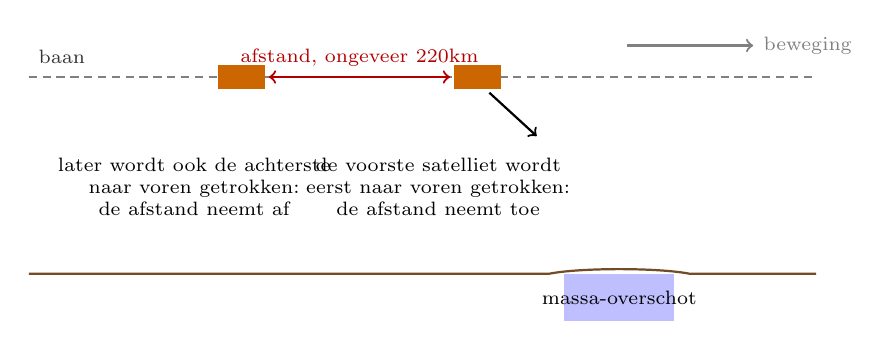
\begin{tikzpicture}[font=\small, x=1cm, y=1cm]
\draw[thick, brown!60!black] (-5,0) -- (1.6,0) .. controls (2.0,0.08) and (3.0,0.08) .. (3.4,0) -- (5,0);
\fill[blue!25] (1.8,0) rectangle (3.2,-0.6);
\node[font=\scriptsize] at (2.5,-0.3) {massa-overschot};
\draw[gray, densely dashed] (-5,2.5) -- (5,2.5);
\node[gray!40!black, font=\scriptsize, anchor=south west] at (-5,2.55) {baan};
\fill[orange!80!black] (-2.6,2.35) rectangle (-2.0,2.65);
\fill[orange!80!black] (0.4,2.35) rectangle (1.0,2.65);
\draw[<->, red!70!black, thick] (-1.95,2.5) -- (0.35,2.5) node[midway, above, font=\scriptsize] {afstand, ongeveer \qty{220}{km}};
\draw[->, thick] (0.85,2.3) -- (1.45,1.75);
\draw[->, thick, gray] (2.6,2.9) -- (4.2,2.9) node[right, font=\scriptsize] {beweging};
\node[font=\scriptsize, anchor=north, align=center] at (0.2,1.6) {de voorste satelliet wordt\\eerst naar voren getrokken:\\de afstand neemt toe};
\node[font=\scriptsize, anchor=north, align=center] at (-2.9,1.6) {later wordt ook de achterste\\naar voren getrokken:\\de afstand neemt af};
\end{tikzpicture}

\par\smallskip{\small Het principe van het satellietpaar (schematisch, niet op
schaal). Bij het naderen van een massa-overschot voelt de voorste satelliet
eerst de aantrekking en wordt naar voren versneld, waardoor de afstand ertussen toeneemt; wanneer
de achterste satelliet boven de massa komt, neemt de afstand weer af. De
afstandsverandering, continu gemeten, wordt omgezet in het zwaartekrachtveld.}
\label{fig:b3:gravity-geodesy:grace}
\end{omfigure}

\begin{omfigure}
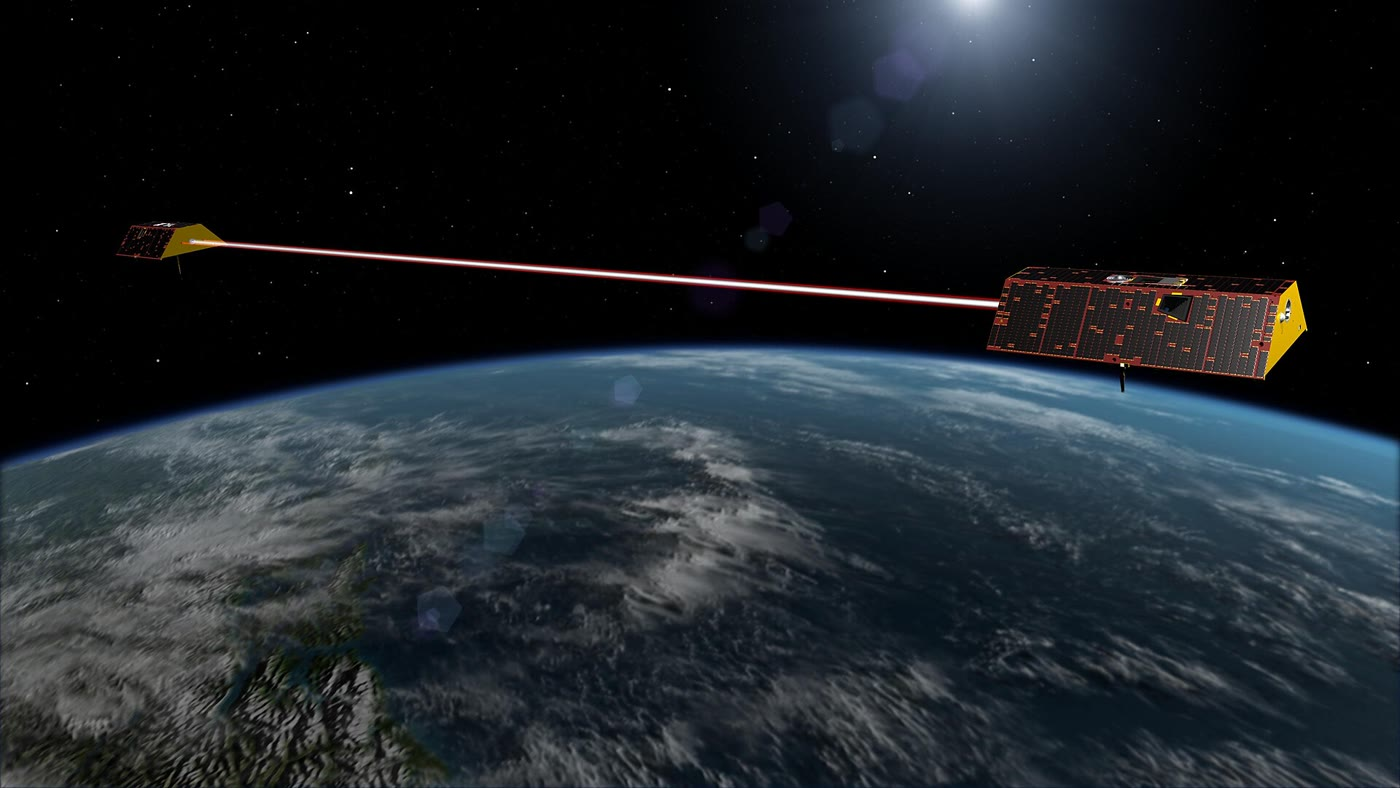
\includegraphics[width=0.66\linewidth]{images/book5/b3-grace-fo-concept.jpg}

\par\smallskip{\small De twee GRACE Follow-On-satellieten, een kunstenaarsweergave (de
afstand tussen hen is sterk verkort). De rode bundel staat voor de
laserafstandsverbinding. NASA/JPL-Caltech, publiek domein.}
\label{fig:b3:gravity-geodesy:grace-photo}
\end{omfigure}

\begin{definition}[Equivalente waterhoogte]\label{def:b3:gravity-geodesy:ewh}
Een verandering van het zwaartekrachtveld die langzaam varieert over afstanden veel groter
dan de dikte van de laag waarin de massa is verplaatst, kan worden voorgesteld als een
verandering van de oppervlaktedichtheid $\sigma$ (\unit{kg.m^{-2}}) op een dunne schil aan het
oppervlak van de Aarde. De \emph{equivalente waterhoogte}\index{equivalente waterhoogte}
is de dikte van zoet water met dezelfde oppervlaktedichtheid:
\[
  h_w = \frac{\sigma}{\rho_w} .
\]
\end{definition}

Een meter water boven een bekken van \qty{1e6}{km^2} is \qty{1e15}{kg}, of
\qty{1000}{Gt}. Het zeeniveau is de andere kant van de rekening: \qty{360}{Gt} ijs
dat aan de oceaan wordt toegevoegd, verhoogt het met ongeveer een millimeter.
% ledger: data:b5-imbie
\omterm{def:b3:gravity-geodesy:satgrav}{Satellietgravimetrie}, satellietaltimetrie en de balans van sneeuwval tegen
ijsafvoer meten elk de massabalans van de ijskappen; samengebracht geven ze
de reeks hieronder.

\begin{omfigure}
\begin{tikzpicture}
\begin{axis}[omrecord, width=0.82\linewidth, height=0.5\linewidth,
  xmin=1992, xmax=2021, ymin=-5600, ymax=600,
  xlabel={jaar}, ylabel={cumulatieve massaverandering (\unit{Gt})},
  xticklabel style={/pgf/number format/1000 sep={}},
  legend pos=south west, legend cell align=left, legend style={font=\scriptsize}]
\addplot[name path=gl, draw=none, forget plot] table[x=year, y=lo] {figdata/out/bachelor-3-ice_mass-greenland.dat};
\addplot[name path=gh, draw=none, forget plot] table[x=year, y=hi] {figdata/out/bachelor-3-ice_mass-greenland.dat};
\addplot[blue!25, forget plot] fill between[of=gl and gh];
\addplot[name path=al, draw=none, forget plot] table[x=year, y=lo] {figdata/out/bachelor-3-ice_mass-antarctica.dat};
\addplot[name path=ah, draw=none, forget plot] table[x=year, y=hi] {figdata/out/bachelor-3-ice_mass-antarctica.dat};
\addplot[red!20, forget plot] fill between[of=al and ah];
\addplot[blue!70!black, thick] table[x=year, y=cum] {figdata/out/bachelor-3-ice_mass-greenland.dat};
\addlegendentry{Groenland}
\addplot[red!70!black, thick] table[x=year, y=cum] {figdata/out/bachelor-3-ice_mass-antarctica.dat};
\addlegendentry{Antarctica}
\draw[gray, densely dotted] (axis cs:2002.25,-5600) -- (axis cs:2002.25,600);
\draw[gray, densely dotted] (axis cs:2017.5,-5600) -- (axis cs:2017.5,600);
\node[font=\scriptsize, gray!40!black, anchor=north] at (axis cs:2009.9,550) {GRACE-jaren};
\end{axis}
\end{tikzpicture}

\par\smallskip{\small Cumulatieve massaverandering van de Groenlandse en Antarctische
ijskappen sinds 1992, met banden van één standaarddeviatie (IMBIE 2021,
samengebrachte schattingen uit altimetrie, gravimetrie en de input--outputmethode). Aan het
eind van 2020 was Groenland $\num{4890} \pm \qty{460}{Gt}$ kwijt en Antarctica
$\num{2670} \pm \qty{530}{Gt}$; rechte-lijnfits geven
\qty{-176}{Gt.yr^{-1}} en \qty{-91}{Gt.yr^{-1}} over 1992--2020, en
\qty{-246}{Gt.yr^{-1}} en \qty{-127}{Gt.yr^{-1}} over de GRACE-jaren.}
\label{fig:b3:gravity-geodesy:ice-mass}
\end{omfigure}

Een zwaartekrachtsanomalie die aan het oppervlak wordt gemeten, is een som van harmonischen; op
de hoogte van een satelliet wordt elke harmonische verzwakt met een factor die van
zijn golflengte afhangt.

\begin{proposition}[Opwaartse voortzetting]\label{prop:b3:gravity-geodesy:upward}
Boven de massa's die haar veroorzaken, is een zwaartekrachtsanomalie die langs het oppervlak
varieert als $\Delta g_0\cos kx$, met $k = 2\pi/\lambda$, op hoogte $z$ (haar
\emph{opwaartse voortzetting}\index{opwaartse voortzetting}) gelijk aan
\[
  \Delta g(x, z) = \Delta g_0\,e^{-kz}\cos kx .
\]
\end{proposition}

\begin{proof}
Boven de massa's voldoet de anomale potentiaal, en daarmee de anomalie, aan
de vergelijking van Laplace $\partial_x^2\Delta g + \partial_z^2\Delta g = 0$. Door de
variabelen te scheiden, volgt $\Delta g = Z(z)\cos kx$ met $Z'' = k^2Z$, waarvan de oplossing die begrensd blijft voor
$z \to \infty$ gelijk aan $Z = \Delta g_0e^{-kz}$.
\end{proof}

Op een hoogte van \qty{400}{km} behoudt een anomalie van \qty{1000}{km} lengte \qty{8}{\percent}
van haar amplitude, een van \qty{100}{km} lengte ongeveer \num{1e-11} ervan:
satellieten zien de lange golflengten, en metingen aan het oppervlak de korte.

\section{Lithosferische buiging}

Boek~3 compenseerde een belasting plaatselijk, waarbij elke kolom op zichzelf dreef.
Een vulkaan op een oceanische plaat wordt niet alleen onder zichzelf gecompenseerd: de
plaat buigt eronder over een breedte van honderden kilometers, en de zeebodem
rond de vulkaan zakt weg in een greppel, waarachter hij omhoog komt in een lage boog.

\begin{definition}[Lithosferische buiging, buigstijfheid, effectieve elastische dikte]\label{def:b3:gravity-geodesy:flexure}
\emph{Lithosferische buiging}\index{lithosferische buiging} is het buigen van de
lithosfeer onder een belasting, gemodelleerd als het buigen van een dunne elastische plaat
die op een vloeibare mantel drijft. De weerstand van de plaat tegen buiging is haar
\emph{buigstijfheid}\index{buigstijfheid}
\[
  D = \frac{ET_e^3}{12(1 - \nu^2)},
\]
en de dikte $T_e$ van de uniforme elastische plaat die buigt zoals de echte
lithosfeer is haar \emph{effectieve elastische dikte}\index{effectieve elastische dikte}.
\end{definition}

\begin{theorem}[Buiging van een dunne plaat]\label{thm:b3:gravity-geodesy:plate}
Een dunne elastische plaat met stijfheid $D$, in één richting gebogen door een belasting $q(x)$
per oppervlakte-eenheid, naar beneden doorgebogen met $w(x)$ en drijvend op een mantel met dichtheid
$\rho_m$, waarbij de holte gevuld is met materiaal met dichtheid $\rho_i$, voldoet aan de
\emph{buigingsvergelijking}\index{buigingsvergelijking}
\[
  D\frac{\mathrm d^4w}{\mathrm dx^4} + (\rho_m - \rho_i)g\,w = q(x) .
\]
\end{theorem}

\begin{proof}
In een gebogen plaat zijn de vezels boven het middenvlak verkort en die eronder
gerekt, evenredig met de kromming $w''$; integratie van de buigspanning
over de dikte geeft het buigmoment $M = -Dw''$, met de
stijfheid uit de definitie (de plaat kan zich niet zijdelings uitzetten, vandaar de factor
$1 - \nu^2$; zie de natuurkundeboeken van jaar 3). Een plakje $\mathrm dx$ van de plaat
draagt op zijn vlakken de dwarskracht $V$ en het moment $M$. Verticaal evenwicht:
de belasting $q\,\mathrm dx$ naar beneden en het drijfvermogen van de verplaatste mantel
$(\rho_m - \rho_i)gw\,\mathrm dx$ naar boven geven $\mathrm dV/\mathrm dx = -q +
(\rho_m - \rho_i)gw$. Momentenevenwicht geeft $\mathrm dM/\mathrm dx = V$.
Dan is $-Dw'''' = M'' = V' = -q + (\rho_m - \rho_i)gw$.
\end{proof}

\begin{definition}[Buigingsparameter, voorwelving]\label{def:b3:gravity-geodesy:alpha}
De \emph{buigingsparameter}\index{buigingsparameter} van een plaat is de
lengte
\[
  \alpha = \left(\frac{4D}{(\rho_m - \rho_i)g}\right)^{1/4},
\]
die de horizontale schaal van haar buiging bepaalt. De \emph{voorwelving}\index{voorwelving}
is de lage boog van opwaartse buiging die een gebogen plaat opricht voorbij de greppel of het
bekken naast haar belasting.
\end{definition}

\begin{proposition}[Lijnbelasting op een doorlopende plaat]\label{prop:b3:gravity-geodesy:line}
Een lijnbelasting $V_0$ per lengte-eenheid langs $x = 0$ buigt de plaat door
\[
  w(x) = w_0e^{-|x|/\alpha}\left(\cos\frac{|x|}{\alpha} + \sin\frac{|x|}{\alpha}\right),
  \qquad w_0 = \frac{V_0\alpha^3}{8D} .
\]
De doorbuiging verdwijnt bij $|x| = 3\pi\alpha/4$, de rand van de greppel; de
top van de \omterm{def:b3:gravity-geodesy:alpha}{voorwelving} ligt bij $|x| = \pi\alpha$, met de hoogte $w_0e^{-\pi} =
\num{0.0432}\,w_0$. Het drijfvermogen van de hele doorbuiging compenseert de belasting:
$\int(\rho_m - \rho_i)gw\,\mathrm dx = V_0$.
\end{proposition}

\begin{proof}
Voor $x > 0$ is de vergelijking $w'''' + 4w/\alpha^4 = 0$; de wortels van
$r^4 = -4/\alpha^4$ zijn $(\pm1 \pm i)/\alpha$, en de oplossingen die ver weg verdwijnen
zijn $e^{-x/\alpha}(A\cos(x/\alpha) + B\sin(x/\alpha))$. Symmetrie legt
$w'(0) = 0$ op, wat $A = B = w_0$ geeft. Integratie van het verticale evenwicht over
de belasting heen: de dwarskracht $V = -Dw'''$ springt met $-V_0$; door symmetrie
is $w'''(0^-) = -w'''(0^+)$, en $w'''(0^+) = 4w_0/\alpha^3$, dus $8Dw_0/\alpha^3 =
V_0$. De doorbuiging verdwijnt waar $\tan(x/\alpha) =
-1$, voor het eerst bij $x = 3\pi\alpha/4$; haar afgeleide,
$-(2w_0/\alpha)e^{-x/\alpha}\sin(x/\alpha)$, verdwijnt daarna bij $x = \pi\alpha$.
Tot slot geldt $\int_0^\infty e^{-u}(\cos u + \sin u)\,\mathrm du = 1$, dus
$\int w\,\mathrm dx = 2w_0\alpha = V_0\alpha^4/(4D) = V_0/((\rho_m - \rho_i)g)$.
\end{proof}

\begin{proposition}[Gebroken plaat]\label{prop:b3:gravity-geodesy:broken}
Een plaat die bij $x = 0$ gebroken is en aan haar vrije uiteinde naar beneden gedrukt wordt, zoals bij een diepzeegreppel,
buigt door als $w = w_0e^{-x/\alpha}\cos(x/\alpha)$ voor $x \ge 0$: de
doorbuiging verdwijnt bij $x = \pi\alpha/2$, en de top van de \omterm{def:b3:gravity-geodesy:alpha}{voorwelving}, de buitenste opheffing,
ligt bij $x = 3\pi\alpha/4$, met de hoogte $w_0e^{-3\pi/4}/\sqrt2 =
\num{0.067}\,w_0$.
\end{proposition}

\begin{proof}
Dezelfde vervallende oplossingen, nu met het vrije uiteinde zonder moment,
$w''(0) = 0$, wat $B = 0$ geeft. Het nulpunt ligt bij $\cos(x/\alpha) = 0$; de
afgeleide $-(w_0/\alpha)e^{-x/\alpha}(\cos + \sin)(x/\alpha)$ verdwijnt bij
$x = 3\pi\alpha/4$, waar $w = w_0e^{-3\pi/4}\cos(3\pi/4)$.
\end{proof}

Afstanden zijn dus de sleutel tot de sterkte van de plaat: meet waar de greppel
eindigt of waar de bult zijn top heeft, dan volgt $\alpha$, daarna $D$, en dan $T_e$.
Omdat $T_e$ als $\alpha^{4/3}$ meetelt, geeft een redelijke schatting van een afstand een goede
van de dikte.

\begin{omfigure}
\begin{tikzpicture}
\begin{groupplot}[group style={group size=1 by 2, vertical sep=1.5cm},
  width=0.82\linewidth, height=0.36\linewidth, xmin=-400, xmax=400,
  tick label style={font=\scriptsize}, label style={font=\small}, title style={font=\small}]
\nextgroupplot[title={(a) lijnbelasting: de Oru-rug op platen van drie diktes},
  ylabel={doorbuiging (\unit{m})}, ymin=-3000, ymax=700, y filter/.expression={-y},
  legend pos=south east, legend cell align=left, legend style={font=\scriptsize}]
\addplot[red!70!black, thick] table[x=x, y=w10] {figdata/out/bachelor-3-flexure-profiles.dat};
\addlegendentry{$T_e = \qty{10}{km}$}
\addplot[blue!70!black, thick] table[x=x, y=w25] {figdata/out/bachelor-3-flexure-profiles.dat};
\addlegendentry{$T_e = \qty{25}{km}$}
\addplot[green!45!black, thick] table[x=x, y=w40] {figdata/out/bachelor-3-flexure-profiles.dat};
\addlegendentry{$T_e = \qty{40}{km}$}
\draw[gray] (axis cs:-400,0) -- (axis cs:400,0);
\draw[->, blue!70!black] (axis cs:222,330) -- (axis cs:222,90);
\node[font=\scriptsize, blue!70!black, anchor=south] at (axis cs:222,330) {voorwelving, $\pi\alpha$};
\nextgroupplot[title={(b) gebroken plaat bij een greppel, $T_e = \qty{25}{km}$},
  xlabel={afstand van de belasting of de greppel (\unit{km})},
  ylabel={doorbuiging (\unit{m})}, xmin=0, xmax=400, ymin=-1100, ymax=280,
  y filter/.expression={-y}]
\addplot[blue!70!black, thick] table[x=x, y=w] {figdata/out/bachelor-3-flexure-broken.dat};
\draw[gray] (axis cs:0,0) -- (axis cs:400,0);
\draw[->] (axis cs:166.5,200) -- (axis cs:166.5,80);
\node[font=\scriptsize, anchor=west] at (axis cs:170,200) {buitenste opheffing, $3\pi\alpha/4$};
\end{groupplot}
\end{tikzpicture}

\par\smallskip{\small Buiging van een elastische plaat (berekend;
$E = \qty{100}{GPa}$, $\nu = 0.25$, mantel \qty{3300}{kg.m^{-3}}, water in de
greppel; verticale schaal sterk overdreven). (a) Onder de belasting van een vulkanische
rug (\qty{4.17e12}{N.m^{-1}}) zinkt een dunne plaat diep en smal, een dikke
ondiep en breed; de \omterm{def:b3:gravity-geodesy:alpha}{voorwelving} verschuift van \qty{112}{km} naar
\qty{316}{km}. (b) Een plaat die bij een greppel is gebroken en met \qty{1}{km} naar beneden is gedrukt:
de buitenste opheffing staat \qty{67}{m} hoog, \qty{167}{km} van de greppel.}
\label{fig:b3:gravity-geodesy:flexure}
\end{omfigure}

\begin{definition}[Regionale isostatische compensatie]\label{def:b3:gravity-geodesy:regional}
\emph{Regionale isostatische compensatie}\index{regionale isostatische compensatie}
is de ondersteuning van een belasting door het drijfvermogen van een doorbuiging die zich uitstrekt over een gebied
breder dan de belasting, via de buigsterkte van de lithosfeer; bij Airy- of
Pratt-compensatie wordt daarentegen elke kolom onder zichzelf gecompenseerd.
\end{definition}

Lokale en regionale compensatie brengen dezelfde totale massa in evenwicht, maar verdelen die
op een andere manier: onder een smalle belasting op een stijve plaat ligt de wortel ondiep en breed,
en de zwaartekrachtsanomalie boven de belasting is sterk positief, geflankeerd door negatieve
anomalieën boven de greppel. Rond de eilanden van de Hawaïaanse rug geven zwaartekracht- en
seismische profielen \omterm{def:b3:gravity-geodesy:flexure}{effectieve elastische diktes} van 17 tot \qty{37}{km}, en
10 tot \qty{20}{km} langs de oudere zeebergen van de Keizerketen, een verschil dat men
uit de ouderdom van de vulkanen en van de plaat die ze belastten verwacht; de waarden
volgen de diepte van een isotherm bij ongeveer
\qty{350}{\degreeCelsius} in de afkoelende oceanische plaat.
% ledger: watts25:te
Dezelfde buiging, onder het gewicht van een bergketen, opent de voorlandbekkens uit Boek~4,
in het hoofdstuk over de Alpiene orogenese.

\begin{omfigure}
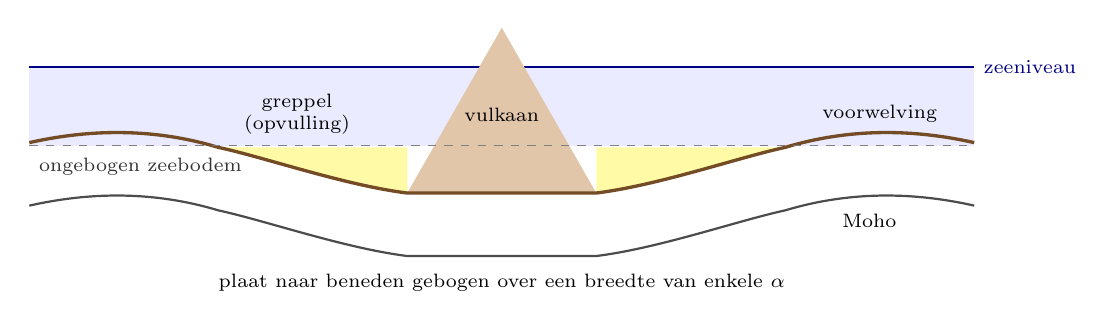
\begin{tikzpicture}[font=\scriptsize, x=1cm, y=1cm]
\fill[blue!8] (-6,0) rectangle (6,-1.0);
\draw[blue!50!black] (-6,0) -- (6,0) node[right] {zeeniveau};
% volcano
\fill[brown!45] (-1.2,-1.6) -- (0,0.5) -- (1.2,-1.6) -- cycle;
% moat infill
\fill[yellow!35] (-1.2,-1.6) .. controls (-2.0,-1.5) and (-3.0,-1.15) .. (-3.6,-1.02) -- (-1.2,-1.02) -- cycle;
\fill[yellow!35] (1.2,-1.6) .. controls (2.0,-1.5) and (3.0,-1.15) .. (3.6,-1.02) -- (1.2,-1.02) -- cycle;
% flexed seafloor (top of crust)
\draw[very thick, brown!60!black] (-6,-0.96) .. controls (-5.2,-0.78) and (-4.4,-0.78) .. (-3.6,-1.02)
  .. controls (-3.0,-1.15) and (-2.0,-1.5) .. (-1.2,-1.6) -- (1.2,-1.6)
  .. controls (2.0,-1.5) and (3.0,-1.15) .. (3.6,-1.02) .. controls (4.4,-0.78) and (5.2,-0.78) .. (6,-0.96);
% Moho, parallel
\draw[thick, gray!60!black] (-6,-1.76) .. controls (-5.2,-1.58) and (-4.4,-1.58) .. (-3.6,-1.82)
  .. controls (-3.0,-1.95) and (-2.0,-2.3) .. (-1.2,-2.4) -- (1.2,-2.4)
  .. controls (2.0,-2.3) and (3.0,-1.95) .. (3.6,-1.82) .. controls (4.4,-1.58) and (5.2,-1.58) .. (6,-1.76);
\node[anchor=west] at (4.2,-1.95) {Moho};
\draw[dashed, gray] (-6,-1.0) -- (6,-1.0);
\node[anchor=north west, gray!40!black] at (-6,-1.03) {ongebogen zeebodem};
\node[anchor=south, align=center] at (-2.6,-0.98) {greppel\\(opvulling)};
\node[anchor=south] at (4.8,-0.82) {voorwelving};
\node at (0,-0.6) {vulkaan};
\node[anchor=north] at (0,-2.5) {plaat naar beneden gebogen over een breedte van enkele $\alpha$};
\end{tikzpicture}

\par\smallskip{\small Een vulkanisch eiland op een oceanische plaat (schematische
dwarsdoorsnede, verticale schaal sterk overdreven). De plaat buigt onder de vulkaan;
de holte eromheen, de greppel, vult zich met vulkanisch puin en sediment, en
verderop stijgt de plaat op in een lage \omterm{def:b3:gravity-geodesy:alpha}{voorwelving}.}
\label{fig:b3:gravity-geodesy:moat}
\end{omfigure}

\begin{inthefield}[Een relatieve zwaartekrachtmeting]
\begin{minipage}[t]{0.55\linewidth}\vspace{0pt}
Een absolute zwaartekrachtmeter laat in een vacuümkamer een hoekkubusspiegel vallen, steeds
opnieuw, en meet de tijd van de val met een laserinterferometer en een atoomklok;
hij geeft de zwaartekracht op één station, maar is zwaar en traag op te zetten. De meting
zelf gebeurt met een relatieve zwaartekrachtmeter, een kleine veerweegschaal die
verschillen in zwaartekracht meet. De geofysicus waterpast hem op een basisplaat bij elk
station van een lijn, leest hem af, noteert de tijd en de hoogte, en gaat verder; elke
paar uur keert de lus terug naar een basisstation, zodat de trage drift van de
veer en de getijden van de vaste Aarde kunnen worden gemeten en verwijderd. Een
satellietontvanger op een paal in de buurt geeft de positie en de hoogte, omdat de zwaartekracht
verandert met ongeveer \qty{0.3}{\milli\gal} per meter hoogte.
\end{minipage}\hfill
\begin{minipage}[t]{0.42\linewidth}\vspace{0pt}
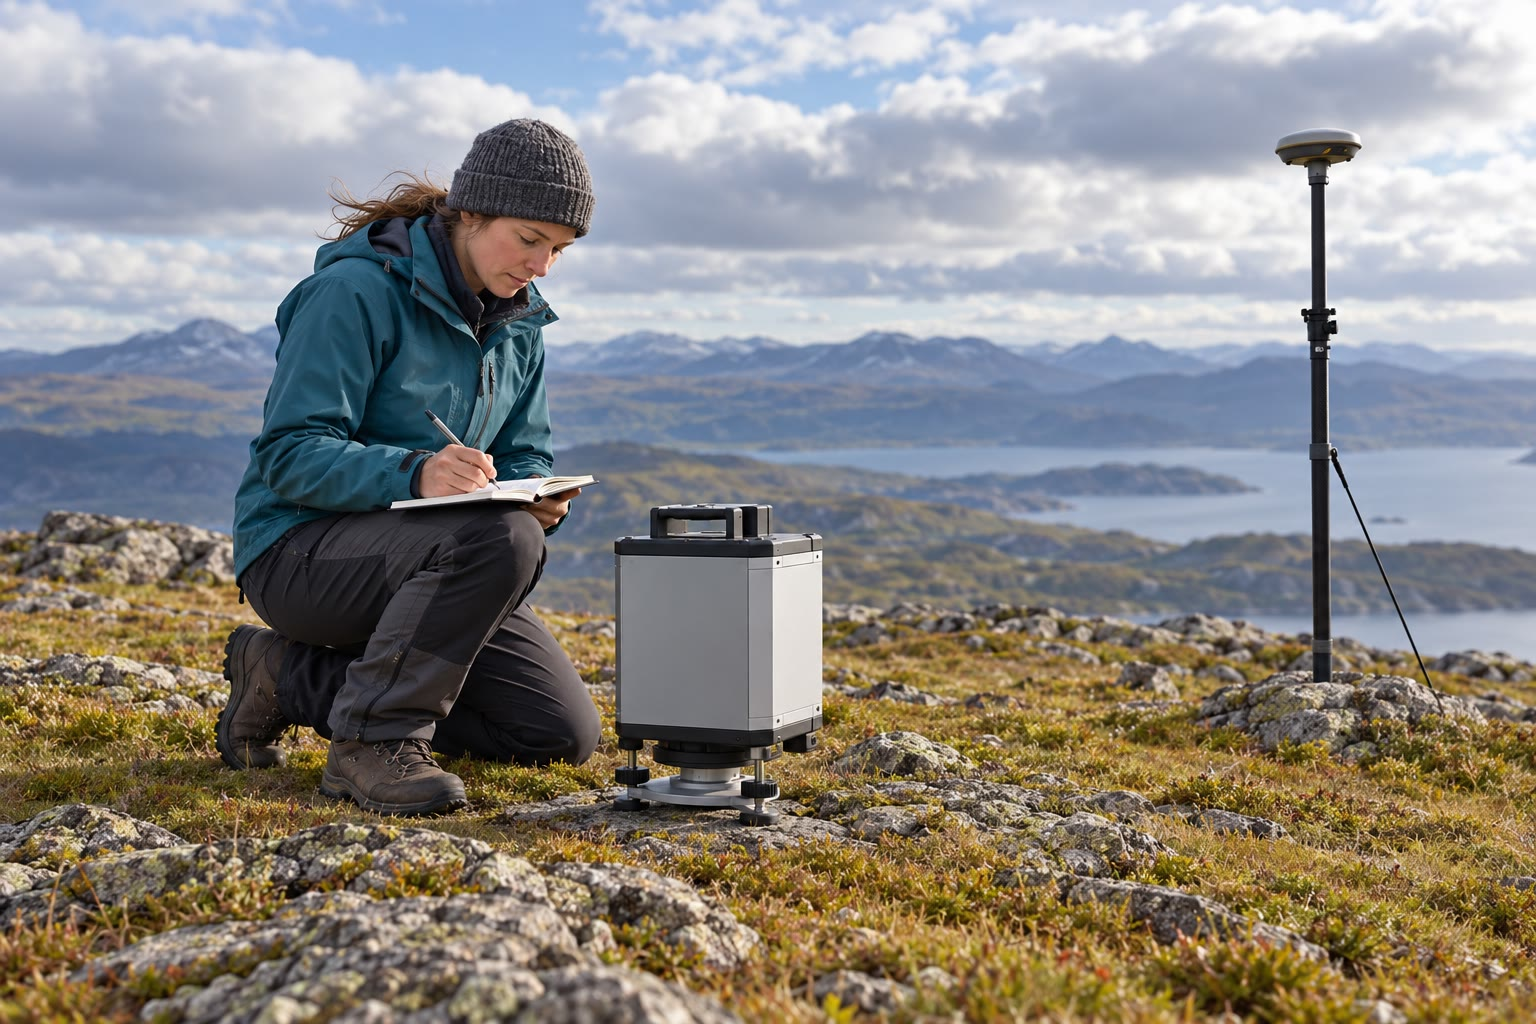
\includegraphics[width=\linewidth]{images/book5/ai/b3-gravimeter.jpg}

{\scriptsize Een veld-zwaartekrachtmeter op zijn waterpasbasis, met op de achtergrond een
satellietantenne (Door AI gegenereerde illustratie.)}
\end{minipage}
\end{inthefield}

\section{Oefeningen}

\begin{exercise}[$\star$]\label{exo:b3:gravity-geodesy:1}
Bereken uit de waarden $a = \qty{6378137}{m}$ en
$f = \num{0.00335281068}$ van het Geodetic Reference System 1980 de halve kleine as $b$ en $a - b$.
Bereken met $J_2 = \num{1.08263e-3}$ en $m = \num{0.00344979}$ de afplatting
die de relatie van Clairaut voorspelt, en vergelijk die.
\end{exercise}

\begin{exercise}[$\star$]\label{exo:b3:gravity-geodesy:2}
In een droog jaar verliest een rivierbekken van \qty{5.0e5}{km^2} \qty{60}{Gt} aan
water. Bereken de verandering van de \omterm{def:b3:gravity-geodesy:ewh}{equivalente waterhoogte}. Schat
hoeveel dezelfde massa het zeeniveau zou doen stijgen, uitgaande van \qty{360}{Gt} per millimeter?
\end{exercise}

\begin{exercise}[$\star$]\label{exo:b3:gravity-geodesy:3}
Met de reeks $\gamma = 9.780327(1 + 0.0053024\sin^2\varphi -
0.0000058\sin^22\varphi)$ \unit{m.s^{-2}}, bereken de normale zwaartekracht aan de evenaar,
bij \ang{45} en aan de polen. Druk het verschil tussen de pool en de evenaar uit in
milligal.
\end{exercise}

\begin{exercise}[$\star$]\label{exo:b3:gravity-geodesy:4}
Bereken de \omterm{def:b3:gravity-geodesy:flexure}{buigstijfheid} en de \omterm{def:b3:gravity-geodesy:alpha}{buigingsparameter} van oceanische platen met
$T_e = \qty{10}{km}$ en $T_e = \qty{30}{km}$ ($E = \qty{100}{GPa}$,
$\nu = 0.25$, $\rho_m - \rho_w = \qty{2270}{kg.m^{-3}}$, $g =
\qty{9.81}{m.s^{-2}}$). Waar liggen de rand van de greppel en de \omterm{def:b3:gravity-geodesy:alpha}{voorwelving} onder een
lijnbelasting?
\end{exercise}

\begin{exercise}[$\star\star$]\label{exo:b3:gravity-geodesy:5}
(a) Bereken bij een geoïdehoogte van $+\qty{50}{m}$ de storingspotentiaal daar,
neem $\gamma = \qty{9.80}{m.s^{-2}}$. (b) Over \qty{100}{km} stijgt de geoïde
met \qty{10}{m}. Met welke hoek wijkt de loodlijn daar af van de normaal op
de ellipsoïde? Geef die in boogseconden.
\end{exercise}

\begin{exercise}[$\star\star$]\label{exo:b3:gravity-geodesy:6}
Uit $J_2 = \num{1.08263e-3}$ en de traagheidsmomentfactor
$C/(Ma^2) = \num{0.3308}$, bereken de dynamische ellipticiteit $H = (C - A)/C$ en
$1/H$. Welk van de twee getallen zou een homogene Aarde met dezelfde $J_2$ veranderen?
\end{exercise}

\begin{exercise}[$\star\star$]\label{exo:b3:gravity-geodesy:7}
Een satelliet vliegt een cirkelbaan \qty{500}{km} boven de equatoriale straal
($a = \qty{6378.137}{km}$, $GM = \qty{3.986005e14}{m^3.s^{-2}}$), met een helling van
\ang{89}. Bereken de omlooptijd en de snelheid van de knooppuntsprecessie in graden per dag.
Waarom kiezen zwaartekrachtmissies bijna-polaire banen?
\end{exercise}

\begin{exercise}[$\star\star$]\label{exo:b3:gravity-geodesy:8}
Twee anomalieën van \qty{10}{\milli\gal} aan het oppervlak hebben golflengten van
\qty{100}{km} en \qty{1000}{km}. Bereken hun amplitudes op \qty{500}{km}
hoogte.
\end{exercise}

\begin{exercise}[$\star\star$]\label{exo:b3:gravity-geodesy:9}
Aan de zeezijde van een oceanische trog ligt de top van de buitenwelving \qty{120}{km} van de
as van de trog. Neem het gebroken-plaatmodel met water boven de plaat en bereken
$\alpha$, $D$ en $T_e$, en de afstand waar de plaat haar ongebogen
niveau kruist.
\end{exercise}

\begin{exercise}[$\star\star\star$]\label{exo:b3:gravity-geodesy:10}
(a) Controleer dat $w = w_0e^{-u}(\cos u + \sin u)$, $u = x/\alpha$, voldoet aan
$Dw'''' + (\rho_m - \rho_i)gw = 0$ voor $x > 0$, met $\alpha$ zoals gedefinieerd.
(b) Toon aan dat het buigmoment $-Dw''$ het grootst is onder de belasting en van teken verandert
bij $x = \pi\alpha/4$. (c) Waar scheurt de plaat het waarschijnlijkst aan
haar bovenzijde, en waarom?
\end{exercise}

\begin{exercise}[$\star\star\star$]\label{exo:b3:gravity-geodesy:11}
Met $m = \num{0.00344979}$ en $C/(Ma^2) = \num{0.3308}$, inverteer de
relatie van Darwin--Radau voor de hydrostatische afplatting. Vergelijk met
$f = \num{0.00335281}$: bereken het verschil en de overhoogte van de
evenaar boven de hydrostatische vorm. Wat zegt dat over de mantel?
\end{exercise}

\begin{exercise}[$\star\star\star$]\label{exo:b3:gravity-geodesy:12}
Een satelliet in een cirkelbaan op \qty{700}{km} hoogte moet het hele jaar dezelfde
oriëntatie ten opzichte van de Zon behouden: zijn knooppunt moet \ang{360} opschuiven
in een tropisch jaar van \num{365.242}~dagen. Bereken de vereiste inclinatie.
\end{exercise}

\section{Probleem: De greppel rond de Orurug}

\begin{problem}[{Weekendprobleem --- de vorm van de Aarde, een vulkanische belasting,
de buigingsgreppel en wat satellieten ervan waarnemen}]
\label{pb:b3:gravity-geodesy:1}
% values: calc/ch03.py; GRS80 (geod5:grs80-*), earth:MoI; flexure.py
Oru is een verzonnen vulkanische rug in een oceaan: een rechte keten van samengegroeide
vulkanen van \qty{400}{km} lang, gebouwd op oude oceanische lithosfeer. Zijn
dwarsdoorsnede wordt aangenomen als een driehoek van \qty{80}{km} breed aan de basis en
\qty{6}{km} hoog, met een dichtheid van \qty{2800}{kg.m^{-3}}, en staat op een zeebodem
\qty{5}{km} diep. Mantel \qty{3300}{kg.m^{-3}}, zeewater
\qty{1030}{kg.m^{-3}}, $E = \qty{100}{GPa}$, $\nu = 0.25$, $g =
\qty{9.81}{m.s^{-2}}$, $G = \qty{6.674e-11}{m^3.kg^{-1}.s^{-2}}$.

\medskip
\noindent\textbf{Deel I --- De vorm van de Aarde.} Gebruik het Geodetic Reference
System 1980: $a = \qty{6378137}{m}$, $b = \qty{6356752.3}{m}$,
$GM = \qty{3.986005e14}{m^3.s^{-2}}$, $J_2 = \num{1.08263e-3}$,
$\omega = \qty{7.292115e-5}{rad.s^{-1}}$, $f = \num{0.00335281}$; en
$C/(Ma^2) = \num{0.3308}$.
\begin{enumerate}
  \item Bereken $m = \omega^2a^2b/(GM)$.
  \item Bereken de afplatting die de relatie van Clairaut geeft uit $J_2$ en
        $m$, en de inverse ervan.
  \item Bereken de hydrostatische afplatting uit de relatie van Darwin--Radau, en
        de inverse ervan.
  \item Vergelijk beide met de waargenomen afplatting. Met hoeveel meter ligt de
        evenaar boven de hydrostatische figuur?
  \item Bereken de dynamische ellipticiteit $H = (C - A)/C$.
\end{enumerate}

\noindent\textbf{Deel II --- De belasting.}
\begin{enumerate}[resume]
  \item Bereken de oppervlakte van de dwarsdoorsnede van de rug.
  \item Bereken de lijnbelasting $V_0$, waarbij de hele rug als ondergedompeld wordt beschouwd, zodat
        ze per volume-eenheid $(\rho_v - \rho_w)g$ weegt.
  \item Als de rug lokaal gecompenseerd zou worden, op de manier van Airy, door een wortel van
        eigen gesteente in de mantel, hoe diep zou die wortel onder de
        top van de rug liggen?
  \item Bij lokale compensatie zou de wortel eindigen aan de voet van de rug,
        \qty{40}{km} van de as. De bathymetrie toont een greppel tot
        \qty{165}{km}. Wat betekent dit?
\end{enumerate}

\noindent\textbf{Deel III --- De buigingsgreppel.} De greppel is gevuld met water
($\rho_i = \rho_w$). Een seismisch profiel over de rug vindt de top van de
oceanische korst weer op zijn regionale diepte \qty{165}{km} van de as, en de
top van de \omterm{def:b3:gravity-geodesy:alpha}{voorwelving} \qty{220}{km} van de as.
\begin{enumerate}[resume]
  \item Bereken de \omterm{def:b3:gravity-geodesy:alpha}{buigingsparameter} uit de rand van de greppel.
  \item Bereken hem opnieuw uit de \omterm{def:b3:gravity-geodesy:alpha}{voorwelving}. Zijn de twee waarden consistent?
  \item Neem $\alpha = \qty{70.0}{km}$ en bereken de \omterm{def:b3:gravity-geodesy:flexure}{buigstijfheid}.
  \item Bereken de \omterm{def:b3:gravity-geodesy:flexure}{effectieve elastische dikte}.
  \item Neem $V_0 = \qty{4.17e12}{N.m^{-1}}$ en $D$ afgerond op drie
        significante cijfers en bereken de doorbuiging onder de as.
  \item Bereken de hoogte van de \omterm{def:b3:gravity-geodesy:alpha}{voorwelving}.
  \item Controleer dat het drijfvermogen van de hele doorbuiging, $2w_0\alpha(\rho_m -
        \rho_w)g$, $V_0$ compenseert.
  \item Vergelijk $T_e$ met de waarden die langs de Hawaïaanse Rug gevonden zijn, 17 tot
        \qty{37}{km}. Vergelijk de doorbuiging onder de as met de
        Airy-wortel van vraag 8.
\end{enumerate}

\noindent\textbf{Deel IV --- Zwaartekracht boven de greppel.} Neem één harmonische van de
buiging, met golflengte $2\pi\alpha$ en amplitude $W = \qty{500}{m}$, die
zowel de zeebodem (korst \qty{2900}{kg.m^{-3}} onder water, \qty{5}{km} onder
zeeniveau) en de Moho (mantel onder de korst, \qty{12}{km} onder zeeniveau) buigt. Een
dun laagje met oppervlaktedichtheid $\sigma$ levert de anomalie $2\pi G\sigma$
net erboven.
\begin{enumerate}[resume]
  \item Bereken de golflengte en het golfgetal $k$ van de harmonische.
  \item Bereken de amplitude van de anomalie op zeeniveau door de doorgebogen
        zeebodem, opwaarts voortgezet vanaf \qty{5}{km} diepte.
  \item Bereken die van de doorgebogen Moho, en de totale waarde.
  \item Bereken de totale waarde op de hoogte van een satelliet, \qty{400}{km} boven
        zeeniveau.
  \item Met welke factor is een harmonische met golflengte \qty{80}{km}, de breedte van
        de rug, op die hoogte verzwakt? Wat kan de satelliet onderscheiden?
  \item Met welke bolharmonische graad $n \approx 2\pi R/\lambda$ komt de
        harmonische van vraag 18 overeen ($R = \qty{6371}{km}$)?
  \item Geef de \omterm{def:b3:gravity-geodesy:flexure}{effectieve elastische dikte} van de plaat onder de
        Orurug.
\end{enumerate}
\end{problem}
